\section{Bayesian Model Averaging (BAM)}
Bayesian Model Averaging is a solution to inference problem with multiple competing models. Suppose data $D$ could correspond to different models $M_k$, $k = 1, \dots, K$, and $\Delta$ is a quantity of interest. We have the posterior distribution:
\begin{equation}
p(\Delta|D) = \sum_{k=1}^K p(\Delta|M_k)\cdot p(M_k|D)
\label{eq:prior_Delta}
\end{equation}
where :
\begin{equation}
p(M_k|D) = \frac{p(D|M_k)\cdot p(M_k)}{\sum_{i=1}^Kp(D|M_i)\cdot p(M_i)}
\end{equation}
and :
\begin{equation}
p(D|M_k) = \int \underbrace{(D|\theta_k,M_k)}_{\text{likelihood}} \cdot p(\theta_k|M_k)d\theta_k
\end{equation}
\newline
This is basically a weighted average of distributions with the weights representing the probability of each model based on the observed data. Averaging over all models provides a better average predictive ability than using any single model $M_j$ conditional on $\mathcal{M} = \left\lbrace M_i : i = 1, \dots , k\right\rbrace$.\\
\newline
One of the tricky parts of this solution is to find the right models to include in our average. Suppose we have a list of models $\mathcal{M} = \left\lbrace M_i : i = 1, \dots , k\right\rbrace$. If $k$ is large, BAM could have a computational cost large as well. We could do a thinning of the models considered for the averaging. Madigan and Raftery proposed two steps to thin the models without losing accuracy.\\
The first step consists of taking in count only the models that are fairly close to the best one, \textit{i.e.} only the models belonging to the following $\mathcal{A}'$:
\begin{equation}
\mathcal{A}' = \left\lbrace M_k:\frac{\max_l\left\lbrace\text{pr}(M_l|D)\right\rbrace}{\text{pr}(M_k|D)}\leq C\right\rbrace
\label{eq:occam_1}
\end{equation}
where $C$ is chosen.\\
\newline
The second step is leaving out the models that are more complicated than another model also in the model list but is less likely to represent the data, \textit{i.e.} we don't consider the models in the following $\mathcal{B}$:
\begin{equation}
\mathcal{B} = \left\lbrace M_k : \exists M_l \in \mathcal{A}', M_l \subset M_k, \frac{\text{pr}(M_l|D)}{\text{pr}(M_k|D)}> 1 \right\rbrace
\label{eq:occam_2}
\end{equation} 
The sum (\ref{eq:prior_Delta}) becomes:
\begin{equation}
p(\Delta|D) = \sum_{M_k \in \mathcal{A}}p(\Delta|D)\cdot p(M_k|D)\text{, }\mathcal{A} := \mathcal{A}'\setminus\mathcal{B}
\label{eq:occam_3}
\end{equation}
This reduces considerably the number of models taken in consideration for the averaging. When a model is rejected, all of his sub-models are rejected too.\\
\newline
In our situation, we want to approximate $p(z|x)$ by $q(z)$, and using the mean-field approximation, we consider that $q(z) = \prod_{j=1}^m q_j(z_j)$. To do so, we use the \textit{CAVI} algorithm and it will give us an optimum for the parameters. The optimum that we obtain is not necessarily a global optimum, as the objective function we are optimizing is not necessarily concave. For example, if we try to find the maxima of the objective function represented in Figure \ref{fig:localOptimum}, depending on where we start, we might find a local maximum that is not global.\\
\newline
\begin{figure}[h!]
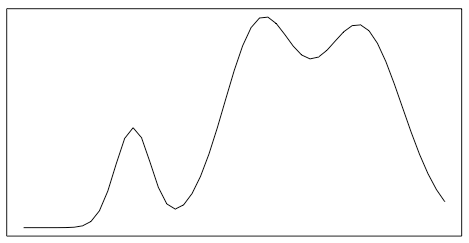
\includegraphics[width=4in]{images/localOptimum.png}
\caption{\label{fig:localOptimum}Depending on the starting parameters for \textit{CAVI} algorithm, it is possible to reach a local optimum that is not global. When using different starting points, the global optimum is reachable.}
\end{figure}
Varying the initialisation of the parameters, we can obtain different optima. We assume that a global optimum exists and is reachable. We compute multiple optima using multiple starting parameters and we obtain different models, each more or less fitting the observed data, this gives us different sets of parameters that represent models $\mathcal{M} = \left\lbrace M_k : k=1, \dots, K\right\rbrace$. \\
\newline
We can then perform a variation of Bayesian Model Averaging on our model set $\mathcal{M}$ to find a distribution of the parameters that would give us a set of parameters corresponding to a model close to the one we are looking for.